%==============================================================================
% Sjabloon poster bachproef
%==============================================================================
% Gebaseerd op document class `a0poster' door Gerlinde Kettl en Matthias Weiser
% Aangepast voor gebruik aan HOGENT door Jens Buysse en Bert Van Vreckem

\documentclass[a0,portrait]{hogent-poster}

% Info over de opleiding
\course{Bachelorproef}
\studyprogramme{toegepaste informatica}
\academicyear{2025-2026}
\institution{Hogeschool Gent, Valentin Vaerwyckweg 1, 9000 Gent}

% Info over de bachelorproef
\title{Automatische notificaties voor nieuwe concerten bij Vlaamse muziekvenues op basis van artiest- en locatievoorkeuren.}
\subtitle{Ontwerp en implementatie van een robuust webscrapingsysteem.}
\author{Kjell Stanssens}
\email{kjell.stanssens@student.hogent.be}
\supervisor{Heidi Roobrouck}
\cosupervisor{Jan Claes (HoGent)}

\specialisation{Full Stack Development}
\keywords{Webscraping, data-extractie, e-mailnotificatiesysteem, veranderingsdetectie, concerten, gebruikersvoorkeuren, notificatievermoeidheid}

\usepackage{tikz}
\usetikzlibrary{shapes,arrows.meta,positioning}
\usepackage{pgfplots}
\pgfplotsset{compat=1.18}

\begin{document}

\maketitle

\large

\begin{abstract}
Deze poster presenteert het onderzoek naar een gepersonaliseerd e-mailnotificatiesysteem voor Vlaamse concertgangers. Versnipperde eventdata leidt vaak tot informatie-overload en gemiste evenementen (Rutten e.a., 2018). Via een robuust webscrapingsysteem worden gebruikers proactief verwittigd op basis van artiest- en locatievoorkeuren. Om notificatievermoeidheid te voorkomen (Mehrotra e.a., 2017), hanteert het systeem een strikt 24-uurs interval.
\end{abstract}

\begin{multicols}{2} 

\section{Inleiding}

Concertinformatie in Vlaanderen is sterk versnipperd over individuele websites. Gebruikers missen evenementen door een gebrek aan efficiënte digitale ontsluiting (Rutten e.a., 2018). Bestaande internationale platformen dekken de lokale markt onvoldoende.

\textbf{Hoofdonderzoeksvraag:} Hoe kan een notificatiesysteem Vlaamse concertgangers tijdig verwittigen, gebaseerd op artiest- en locatievoorkeuren (Graves, 2003), zonder disruptief te zijn?

\textbf{Deelvragen:}
\begin{itemize}
    \item \textit{Probleemdomein:} Welke metadata zijn essentieel voor concertnotificaties en wat zijn de tekortkomingen van platformen zoals Bandsintown of Songkick?
    \item \textit{Oplossingsdomein:} Welke data-architectuur en scraping-frameworks zijn vereist om een schaalbaar en betrouwbaar systeem te realiseren?
\end{itemize}

\section{Materialen en Methode}

Het technische ontwerp combineert een asynchrone \textit{FastAPI}-backend met een \textit{Celery}-taakwachtrij voor achtergrondverwerking. De modulaire pijplijn is als volgt gestructureerd:

\begin{center}
  \captionsetup{type=figure}
  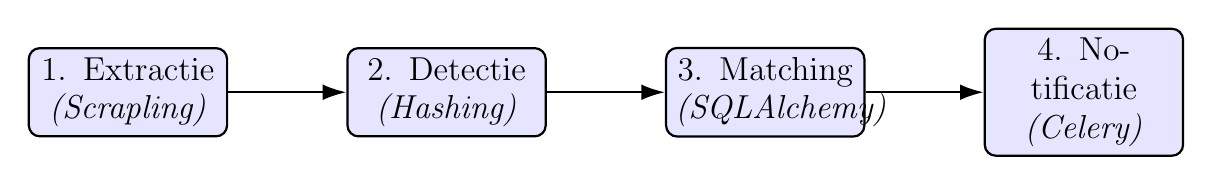
\begin{tikzpicture}[
      node distance=1.8cm and 1.5cm, 
      auto, 
      thick, 
      every node/.style={font=\large},
      block/.style={rectangle, draw, fill=blue!10, text width=6.5em, text centered, rounded corners, minimum height=3em},
      line/.style={draw, -{Latex[length=3mm, width=2mm]}}
    ]
    % Nodes
    \node [block] (scrape) {1. Extractie\\ \textit{(Scrapling)}};
    \node [block, right=of scrape] (hash) {2. Detectie\\ \textit{(Hashing)}};
    \node [block, right=of hash] (match) {3. Matching\\ \textit{(SQLAlchemy)}};
    \node [block, right=of match] (notif) {4. Notificatie\\ \textit{(Celery)}};
    % Lines
    \path [line] (scrape) -- (hash);
    \path [line] (hash) -- (match);
    \path [line] (match) -- (notif);
  \end{tikzpicture}
  \captionof{figure}{Geautomatiseerde gegevensstroom: van extractie tot notificatie}
\end{center}

\section{Resultaten}

\begin{center}
  \captionsetup{type=figure}
  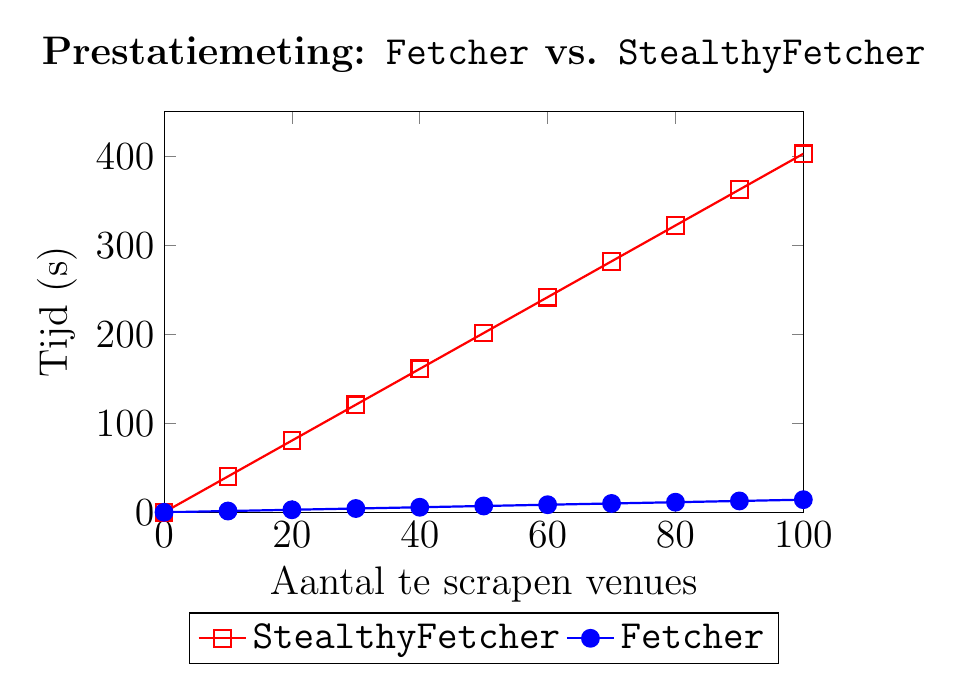
\begin{tikzpicture}
      \begin{axis}[
          width=0.8\linewidth,
          height=0.55\linewidth,
          title={Prestatiemeting: \texttt{Fetcher} vs. \texttt{StealthyFetcher}},
          xlabel={Aantal te scrapen venues},
          ylabel={Tijd (s)},
          xmin=0, xmax=100,
          ymin=0, ymax=450,
          xtick={0, 20, 40, 60, 80, 100},
          ytick={0, 100, 200, 300, 400},
          grid style=dashed,
          mark size=3pt,
          title style={font=\Large\bfseries, yshift=1ex},
          label style={font=\Large},
          tick label style={font=\Large},
          legend style={at={(0.5,-0.25)}, anchor=north, legend columns=-1, font=\Large}      ]
      
      % Data voor Stealthy Fetcher
      \addplot[color=red, mark=square, thick]
      coordinates {
          (0, 0.00) (10, 40.28) (20, 80.55) (30, 120.83) 
          (40, 161.10) (50, 201.38) (60, 241.66) (70, 281.93) 
          (80, 322.21) (90, 362.48) (100, 402.76)
      };
      \addlegendentry{\texttt{StealthyFetcher}}

      % Data voor Standaard Fetcher
      \addplot[color=blue, mark=*, thick]
      coordinates {
          (0, 0.00) (10, 1.42) (20, 2.83) (30, 4.25) 
          (40, 5.66) (50, 7.08) (60, 8.50) (70, 9.91) 
          (80, 11.33) (90, 12.74) (100, 14.16)
      };
      \addlegendentry{\texttt{Fetcher}}
      
      \end{axis}
  \end{tikzpicture}
  \captionof{figure}{Uitvoeringstijd in seconden. De \texttt{Fetcher} op de netwerklaag presteert significant efficiënter dan extractie via de applicatielaag.}
\end{center}

\vspace{0.5cm}

Uit de deterministische testsuite binnen het Pytest-framework blijkt:
\begin{itemize}
    \item \textbf{Schaalbaarheid (KPI 1):} De extractielaag is 100\% configuratie-gestuurd via JSON-gekoppelde schema's.
    \item \textbf{Notificatie-interval (KPI 2):} Opeenvolgende triggers worden succesvol gebundeld tot maximaal één e-mail per 24 uur.
    \item \textbf{Precisie (KPI 3):} De matching-engine behaalt een nauwkeurigheid van 100\% zonder false positives.
\end{itemize}

\section{Besluit en Discussie}

Het ontwikkelde prototype bewijst dat gecentraliseerde monitoring van een versnipperde markt technisch en ethisch haalbaar is.

\textbf{Voor de gebruiker en de sector:}
\begin{itemize}
    \item \textbf{Tijdsbesparing:} Handmatige controle van 5 tot 10 websites is overbodig. Gebundelde notificaties elimineren notificatievermoeidheid (Mehrotra e.a., 2017).
    \item \textbf{Fair-use:} Volledige naleving van de AVG en \texttt{robots.txt} (Bereczki \& Liber, 2024). Het systeem concurreert niet met ticketverkoop en stuurt verkeer direct naar de bronorganisatie (Krotov \& Silva, 2018).
\end{itemize}

\textbf{Implicaties voor het onderzoeksdomein:} \\
Dit onderzoek toont aan dat configuratie-gestuurde netwerkextractie een robuust alternatief biedt wanneer publieke API's ontbreken. Toekomstig onderzoek kan dit model uitbreiden door muzikale voorkeuren te koppelen aan geografische reisafstand (Zangerle e.a., 2018), om zo impliciete contextuele aanbevelingen te genereren.

\section{Referenties}
\begingroup
\small
\begin{itemize}
    \item Bereczki, T. \& Liber, Á. (2024). \textit{The state of web scraping in the EU}. International Association of Privacy Professionals.
    \item Graves, M. J. (2003). \textit{Concert Event Metadata: Describing Concerts Effectively in a Digital Environment} (Masterscriptie). University of North Carolina.
    \item Krotov, V. \& Silva, L. (2018). Legality and Ethics of Web Scraping. \textit{AMCIS}.
    \item Mehrotra, A., e.a. (2017). \textit{Intelligent Notification Systems: A Survey of the State of the Art}. arXiv:1711.10171.
    \item Rutten, K., e.a. (2018). \textit{De digitale transitie is mensenwerk: hergebruik van digitale culturele content}. Universiteit Gent.
    \item Zangerle, E. e.a. (2018). Content-based User Models: Modeling Music Preferences and Concert Attendance. \textit{ISMIR}.
\end{itemize}
\endgroup

\end{multicols}
\end{document}